\begin{figure}[t]
\centering
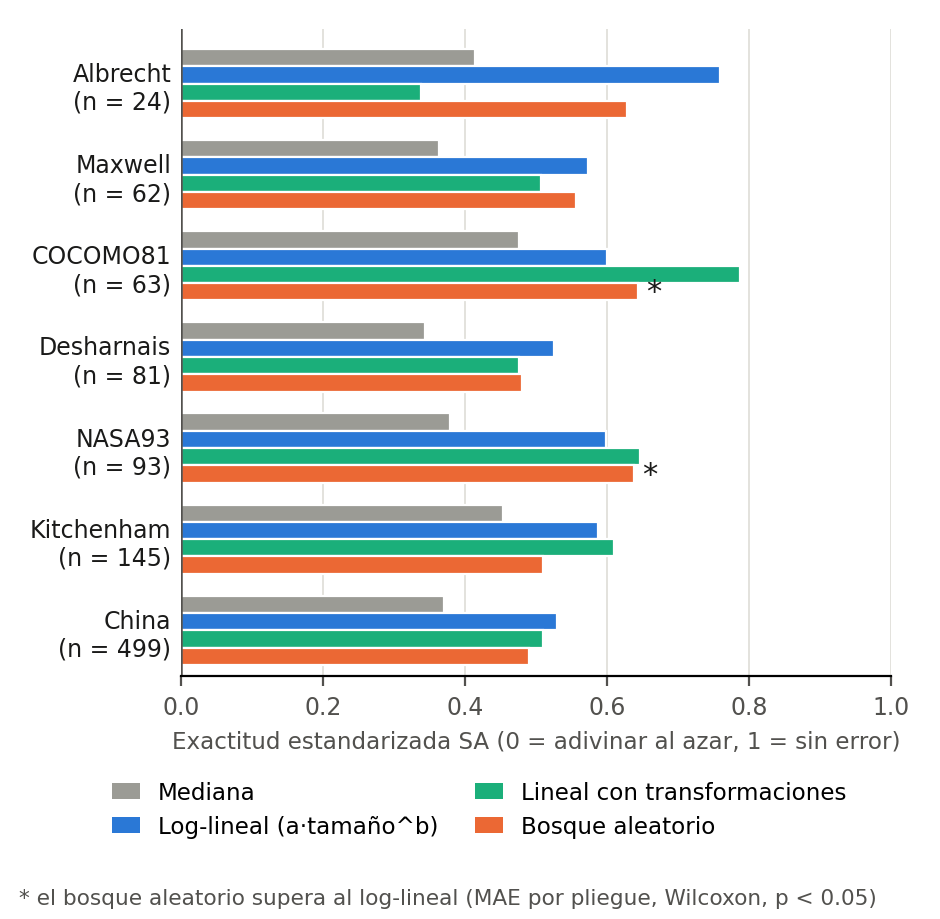
\includegraphics[width=0.95\linewidth]{../outputs/figures/fig3_sa_modelos.png}
\caption{Exactitud estandarizada (SA) promedio de los cuatro modelos en cada dataset, de los que tienen menos proyectos (arriba) a los que tienen m\'as (abajo). Cero equivale a adivinar al azar y uno a no tener error. El asterisco marca los datasets donde el bosque aleatorio supera al log-lineal ($p<0.05$).}
\label{fig:sa}
\end{figure}

\begin{figure}[t]
\centering
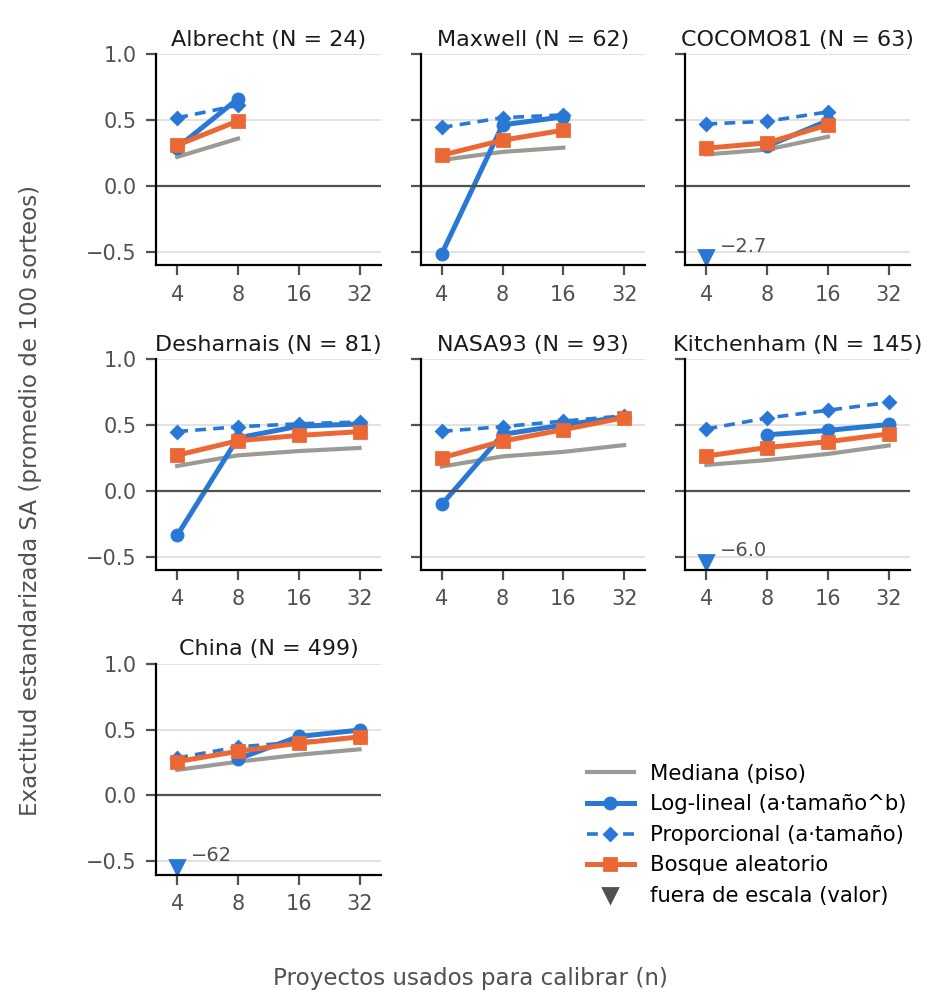
\includegraphics[width=0.95\linewidth]{../outputs/figures/fig4_curva_aprendizaje.png}
\caption{Curvas de aprendizaje: SA promedio de 100 sorteos con $n$ proyectos de entrenamiento y el resto del dataset como prueba. Gris: mediana (el piso). Azul continuo: log-lineal. Azul discontinuo: modelo proporcional, que solo calibra $a$. Naranja: bosque aleatorio. Los tri\'angulos al pie marcan promedios fuera de escala, con su valor.}
\label{fig:curva}
\end{figure}

\begin{figure}[t]
\centering
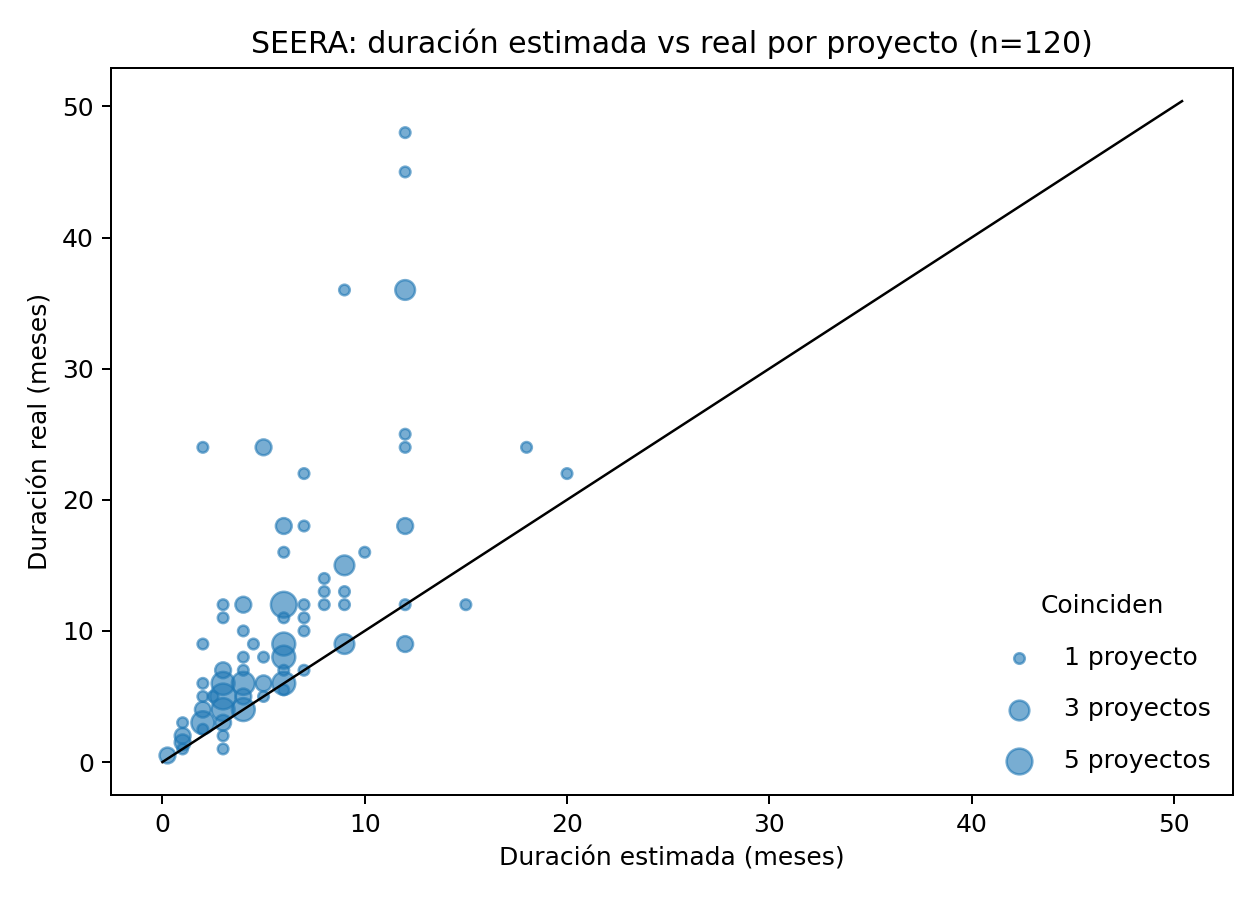
\includegraphics[width=0.95\linewidth]{../outputs/figures/fig5_seera_duracion.png}
\caption{Duraci\'on estimada contra duraci\'on real por proyecto en SEERA. Los puntos por encima de la diagonal son proyectos que tardaron m\'as de lo estimado; el \'area de cada punto indica cu\'antos proyectos coinciden en ese par. En SEERA el esfuerzo se calcula a partir de la duraci\'on, por eso sus desviaciones coinciden con las del esfuerzo.}
\label{fig:seeradur}
\end{figure}
